\documentclass[10pt,pdf,hyperref={unicode}]{beamer}


%\documentclass[10pt]{beamer}

\usetheme[progressbar=frametitle]{metropolis}

\usepackage{booktabs}
\usepackage[scale=2]{ccicons}

\usepackage{pgfplots}

\usepgfplotslibrary{dateplot}

\usepackage{xspace}
\newcommand{\themename}{\textbf{\textsc{metropolis}}\xspace}

\usepackage{multicol}
%\usepackage{lmodern}

% подключаем кириллицу 
\usepackage[T2A]{fontenc}
\usepackage[utf8]{inputenc}
\usepackage{listings}
%\usepackage{graphicx}
\usepackage{hyperref}

% отключить клавиши навигации
\setbeamertemplate{navigation symbols}{}

% тема оформления
\usetheme{Pittsburgh}

% цветовая схема
\usecolortheme{default}

\definecolor{light-gray}{gray}{0.90}

\title{Семинар №11}   
\subtitle{ФАКТ \the\year}
\author{Бирюков В. А.} 
\date{\today}
% \logo{
\includegraphics[height=5mm]{images/logo.png}\vspace{-7pt}}

\begin{document}

\lstset{language=C}

% титульный слайд
\begin{frame}
\titlepage
\end{frame} 

\lstset{
  language=C++,                % choose the language of the code
  basicstyle=\linespread{1.1}\ttfamily,
  columns=fixed,
  fontadjust=true,
  basewidth=0.5em,
  keywordstyle=\color{blue}\bfseries,
  commentstyle=\color{gray},
  stringstyle=\ttfamily\color{orange!50!black},
  showstringspaces=false,
  numbersep=5pt,
  numberstyle=\tiny\color{black},
  numberfirstline=true,
  stepnumber=1,                   % the step between two line-numbers.        
  numbersep=10pt,                  % how far the line-numbers are from the code
  backgroundcolor=\color{black!2},  % choose the background color. You must add \usepackage{color}
  showstringspaces=false,         % underline spaces within strings
  captionpos=b,                   % sets the caption-position to bottom
  breaklines=true,                % sets automatic line breaking
  breakatwhitespace=true,         % sets if automatic breaks should only happen at whitespace
  xleftmargin=.2in,
  extendedchars=\true,
  keepspaces = true,
}
\lstset{literate=%
   *{0}{{{\color{red!20!violet}0}}}1
    {1}{{{\color{red!20!violet}1}}}1
    {2}{{{\color{red!20!violet}2}}}1
    {3}{{{\color{red!20!violet}3}}}1
    {4}{{{\color{red!20!violet}4}}}1
    {5}{{{\color{red!20!violet}5}}}1
    {6}{{{\color{red!20!violet}6}}}1
    {7}{{{\color{red!20!violet}7}}}1
    {8}{{{\color{red!20!violet}8}}}1
    {9}{{{\color{red!20!violet}9}}}1
}

\newcommand{\imageSizeMult}{1}

\section{Полиморфизм}

\begin{frame}[fragile]
\frametitle{Полиморфизм: Структура базового класса}
\begin{lstlisting}
class Animal {
protected:
    std::string mName;
    int mAge;
public:
    Animal(std::string name, int age) 
    	: mName(name), mAge(age) {}

    void say() const {
        cout << "<abstract sounds>" << endl;
    }
    void move() const {
        cout << "<abstract walking>" << endl;
    }
};
\end{lstlisting}
\end{frame}


\begin{frame}[fragile]
\frametitle{Полиморфизм: Структура класса наследника}
\begin{lstlisting}
class Cat : public Animal {
private:
    int mMiceCaught;
public:
    Cat(std::string name, int age, int miceCaught) 
    : Animal(name, age), mMiceCaught(miceCaught) 
    {}

    void say() const {
        cout << "Meow!" << endl;
    }
    void move() const {
        cout << "<sneaking>" << endl;
    }
};
\end{lstlisting}
\end{frame}


\begin{frame}[fragile]
\frametitle{Полиморфизм: представление объектов в памяти}
\begin{center}
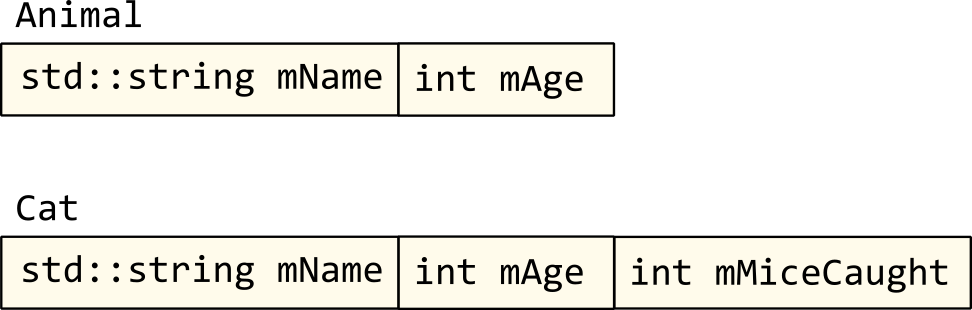
\includegraphics[width=\imageSizeMult\linewidth]{../images/classes_representation.png}
\end{center}
\end{frame}


\begin{frame}[fragile]
\frametitle{Указатель базового класса на объект базового класса}
\begin{center}
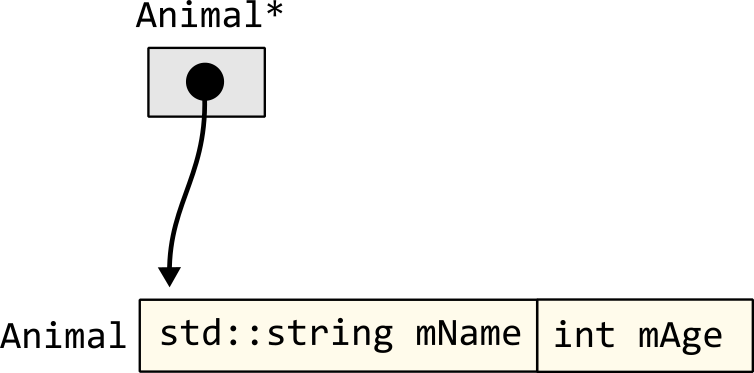
\includegraphics[width=0.7\linewidth]{../images/animal_pointer_to_animal.png}
\end{center}
\end{frame}

\begin{frame}[fragile]
\frametitle{Указатель базового класса на объект класса наследника}
\begin{center}
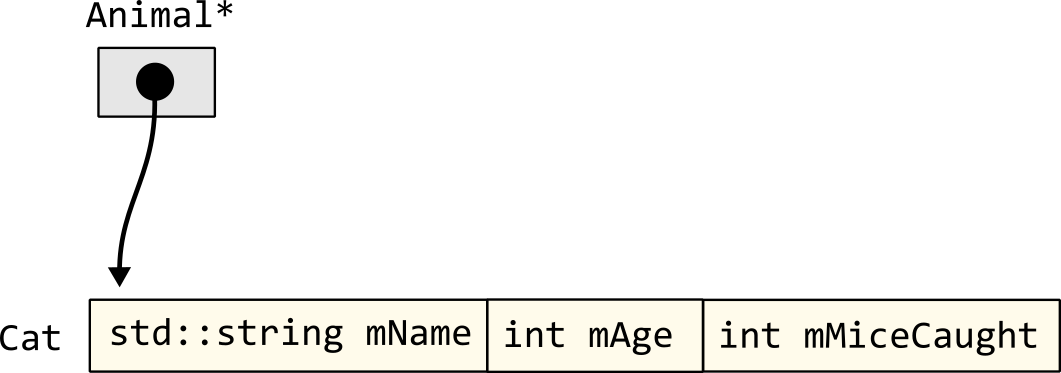
\includegraphics[width=\imageSizeMult\linewidth]{../images/animal_pointer_to_cat.png}
\end{center}
\end{frame}


\section{Добавим виртуальные функции}

\begin{frame}[fragile]
\frametitle{Таблица виртуальных функций}
\begin{itemize}
\item Реализация полтморфизма не задаётся стандартом
\item Но почти всегда используется таблица виртуальных функций
\end{itemize}
\end{frame}

\begin{frame}[fragile]
\frametitle{Сделаем методы виртуальными}
\begin{lstlisting}
class Animal {
protected:
    std::string mName;
    int mAge;
public:
    Animal(std::string name, int age) 
    	: mName(name), mAge(age) {}

    virtual void say() const {
        cout << "<abstract sounds>" << endl;
    }
    virtual void move() const {
        cout << "<abstract walking>" << endl;
    }
};
\end{lstlisting}
\end{frame}

\begin{frame}[fragile]
\frametitle{Указатель базового класса на объект базового класса}
\begin{center}
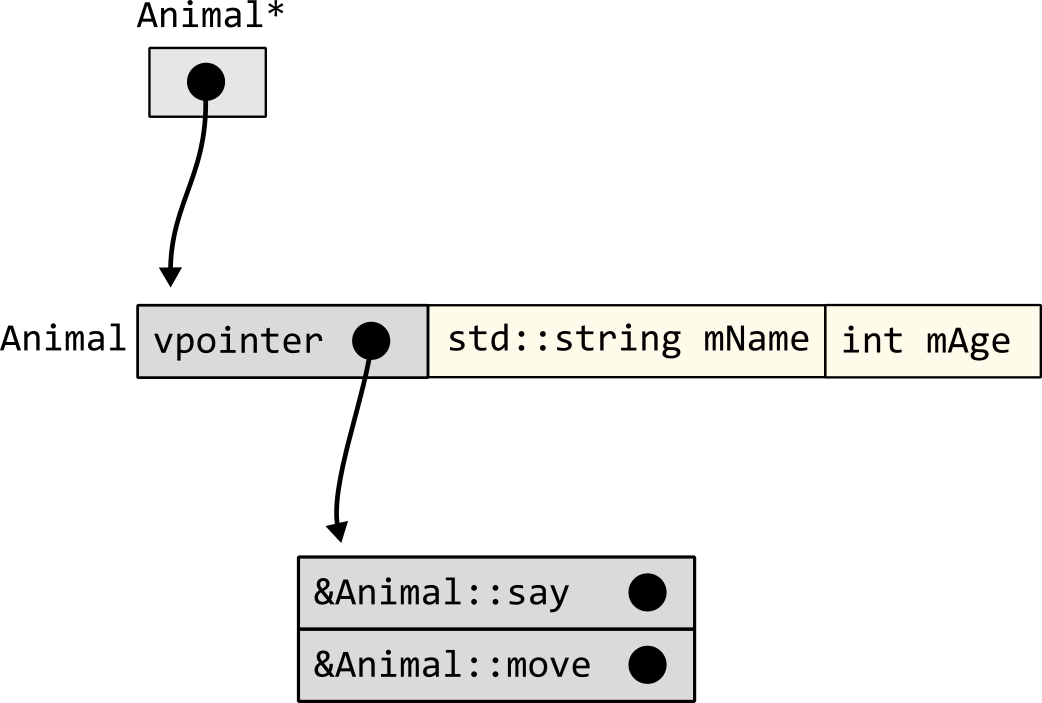
\includegraphics[width=0.8\linewidth]{../images/virtual_animal_pointer_to_animal.png}
\end{center}
\end{frame}



\begin{frame}[fragile]
\frametitle{Указатель базового класса на объект класса наследника}
\begin{center}
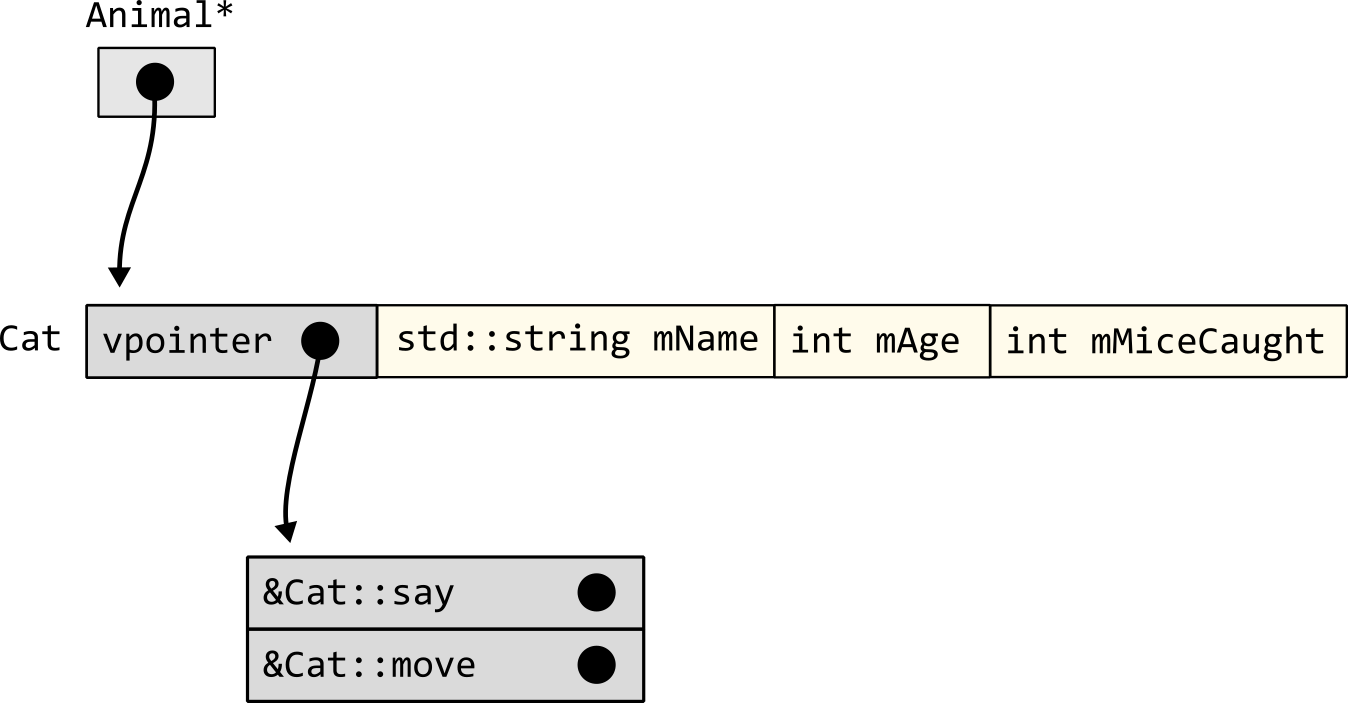
\includegraphics[width=\imageSizeMult\linewidth]{../images/virtual_animal_pointer_to_cat.png}
\end{center}
\end{frame}


\begin{frame}[fragile]
\frametitle{Динамический тип}
\begin{lstlisting}
Cat cat {"Cleo", 10, 100};
Animal* p = &cat;
\end{lstlisting}

\begin{itemize}
\item Статический тип \texttt{p} -- указатель на Animal
\item Динамический тип \texttt{p} -- указатель на Cat
\end{itemize}

\end{frame}



\end{document}
